\documentclass[9pt,aspectratio=169]{beamer}

\usepackage{tabularx}
\newcolumntype{Y}{>{\centering\arraybackslash\leavevmode}X}
\usepackage{luamplib}
\mplibsetformat{metafun}
\mplibtextextlabel{enable}
\everymplib{input repere; input macros; beginfig(1);}
\everyendmplib{endfig;}

\usetheme{graham}

\title{Angles and Triangles}
\subtitle[Graham Middle School]{Graham Middle School Math Olympiad Team}

\begin{document}
\maketitle

\begin{frame}{Elements}
  \begin{columns}[T]
    \begin{column}{0.5\textwidth}
      \begin{wrapfigure}[8]{r}{0.23\textwidth}
        \vspace*{-1.2\baselineskip}
        \hspace*{-1em}
        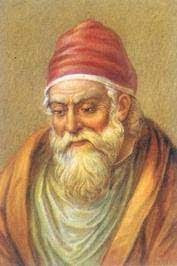
\includegraphics[width=0.28\textwidth]{10 - Angles and Triangles/euclid.jpg}
      \end{wrapfigure}
      2320~years~ago,~Greek~mathematician \emph{Euclid of Alexandria} published \textbf{Elements}, the most influential non-religion book in history. In his book was about geometry Euclid split statements into \emph{definitions}, \emph{axioms}, and \emph{propositions}. This approach influenced almost any aspect of our life: from law to logic and modern science. Euclid started from definitions of the simplest figures: 
      \begin{definition}
        a \textbf{point} (is that which has position but not dimensions), 
        
        a \textbf{line} (is length without breadth), and 
        
        a \textbf{plane} (is that which has length and breadth).
      \end{definition}
      Then he gave some axioms and postulates, statements that we accept without proof.

      After that he gave \textbf{mathematical proofs} of the propositions.
    \end{column}
    \begin{column}{0.5\textwidth}
      Some of the axioms reformulated by \textbf{Hilbert} (who helped Einstein with relativity theory equations):
      \begin{definition}
        \emph{For every \textbf{two points}, there exists exactly \textbf{one line} that contains them both.} 
        
        \emph{There exist at least \textbf{two} points on a \textbf{line}. There exist at least \textbf{three} points that do \textbf{not} lie on a line.}
        
        \emph{There exists at least \textbf{one} point between \textbf{two points} of a line.}

        And the most famous (the fifth postulate of Euclid):

        \emph{For a line and a point not on a line, there is exactly \textbf{one line} in the plane that passes through the point and does \textbf{not intersect} given line} (a parallel line).
      \end{definition}
      Most of the other axioms are about a plane and how to \emph{measure segments} and \emph{angles}.
      \begin{example}
        The irony is that modern geometry doesn't define points, lines, and planes. So points, lines, and planes now are anything that satisfies the set of axioms.
      \end{example}
    \end{column}
  \end{columns}
\end{frame}

\begin{frame}{Types of angles and their measures}
  \begin{columns}[T]
    \begin{column}{0.5\textwidth}
      We typically measure angles in degrees (symbol~$°$), with an entire circle having a measure of $360°$.  A pair of rays intersecting to form a~straight line therefore form a $180°$ angle. The number $360$ is somewhat arbitrary.  It was developed in ancient Babylonia where they used a sexigesimal (base $60$) number system and had a $360$ day calendar.

      \begin{example}
        Angles are sometimes also measured in radians, where $2\pi$ radians is equal to $360$ degrees.
      \end{example}

      Angles are usually denoted with small greek letters. The most commonly used letters for angles are $\alpha$ (alpha), $\beta$ (beta), $\gamma$ (gamma), $\theta$~(theta), $\phi$ (phi), and $\psi$ (psi). Also, the letter $\pi$ (pi) is used to denote an angle $180°$.
    \end{column}
    \begin{column}{0.5\textwidth}
      Angles are classified as acute, right, or obtuse depending on whether they measure less than, equal to, or greater than $90°$ respectively.\medskip

      \begin{tabularx}{\textwidth}{YYY}
        \begin{mplibcode}
          u = 0.6cm;
          repere(-1,5,u,-1,5,u);
            drawarrow (0, 0)--(2 * dir(40)) withpen pencircle scaled 1.25;
            drawarrow (0, 0)--(2, 0) withpen pencircle scaled 1.25;
            pickup pencircle scaled 2.5;
            drawdot (0, 0);
          fin;
        \end{mplibcode}
        &
        \begin{mplibcode}
          u = 0.6cm;
          repere(-1,5,u,-1,5,u);
            drawarrow (0, 0)--(2 * dir(90)) withpen pencircle scaled 1.25;
            drawarrow (0, 0)--(2, 0) withpen pencircle scaled 1.25;
            draw marqueangledroit((2, 0), (0, 0), (0, 2));
            pickup pencircle scaled 2.5;
            drawdot (0, 0);
          fin;
        \end{mplibcode}
        &
        \begin{mplibcode}
          u = 0.6cm;
          repere(-1,5,u,-1,5,u);
            drawarrow (0, 0)--(2 * dir(120)) withpen pencircle scaled 1.25;
            drawarrow (0, 0)--(2, 0) withpen pencircle scaled 1.25;
            pickup pencircle scaled 2.5;
            drawdot (0, 0);
          fin;
        \end{mplibcode} \\
        Acute & Right & Obtuse
      \end{tabularx}
      \begin{definition}
        Pairs of angles whose measures sum to $90°$ are called \textbf{complementary} angles.  
        
        Pairs of angles that sum to $180°$ are called \textbf{supplementary}.
      \end{definition}\medskip

      \begin{tabularx}{\textwidth}{YY}
        \begin{mplibcode}
          u = 0.6cm;
          repere(-5,5,u,-1,5,u);
            draw marqueangle(dir(40), (0, 0), (0,2), 1);
            draw marqueangle((2,0), (0, 0), dir(40), 2);
            drawarrow (0, 0)--(2 * dir(40)) withpen pencircle scaled 1.25;
            drawarrow (0, 0)--(2 * dir(90)) withpen pencircle scaled 1.25;
            drawarrow (0, 0)--(2, 0) withpen pencircle scaled 1.25;
            draw marqueangledroit((0, 2), (0, 0), (-2, 0));
            draw (0, 0)--(-2, 0);
            pickup pencircle scaled 2.5;
            drawdot (0, 0);
          fin;
        \end{mplibcode}
        &
        \begin{mplibcode}
          u = 0.6cm;
          repere(-5,5,u,-1,5,u);
            draw marqueangle(dir(70), (0, 0), (-2,0), 1);
            draw marqueangle((2,0), (0, 0), dir(70), 2);
            drawarrow (0, 0)--(2 * dir(70)) withpen pencircle scaled 1.25;
            drawarrow (0, 0)--(-2, 0) withpen pencircle scaled 1.25;
            drawarrow (0, 0)--(2, 0) withpen pencircle scaled 1.25;
            pickup pencircle scaled 2.5;
            drawdot (0, 0);
          fin;
        \end{mplibcode} \\
        Complementary & Supplementary 
      \end{tabularx}

    \end{column}
  \end{columns}
\end{frame}

\begin{frame}{Vertical angles and angles formed by parallel lines}
  \begin{columns}[T]
    \begin{column}{0.5\textwidth}
      \begin{center}
        \leavevmode
        \begin{mplibcode}
          u = 1cm;
          repere(-5,5,u,-5,5,u);
            pair O, A, B, C, D;
            O := (0, 0);
            A := (2 * dir(25));
            B := (2 * dir(-25));
            C := (-2 * dir(25));
            D := (-2 * dir(-25));
            drawarrow O--A withpen pencircle scaled 1.25;
            drawarrow O--B withpen pencircle scaled 1.25;
            drawarrow O--C withpen pencircle scaled 1.25;
            drawarrow O--D withpen pencircle scaled 1.25;
            pickup pencircle scaled 2.5;
            drawdot O;
            nomme(B, O, A, btex $\phi$ etex);
            nomme(D, O, C, btex $\phi'$ etex);
            label.top(btex $\theta$ etex, O + 0.15 * dir(90));
            label.bot(btex $\theta'$ etex, O + 0.15 * dir(-90));
          fin;
        \end{mplibcode}
      \end{center}

      Two pairs of vertical angles ($\theta$ and $\theta'$, $\phi$ and $\phi'$) are formed by intersecting lines.  Since they are angles that make a line, $\theta$ and $\phi$ sum to $180°$.  Likewise, $\theta'$ and $\phi$ sum to $180°$.  Therefore $\theta = \theta'$ and the angles are said to be congruent.  Since $\phi$ and $\phi'$ both form lines when combined with $\theta$, we also see that $\phi = \phi'$.

      \begin{definition}
        Intersecting lines form two pairs of congruent \textbf{vertical} angles.
      \end{definition}

    \end{column}
    \begin{column}{0.5\textwidth}
      In the figure below, $l$ and $m$ are parallel lines and line $n$ is called a \textbf{transversal}.  
      \begin{center}
        \leavevmode
        \begin{mplibcode}
          u = 0.4cm;
          repere(-5,5,u,-5,5,u);
            path l, m, n;
            l := (-5, 1.5)--(5, 1.5);
            m := (-5, -1.5)--(5, -1.5);
            n := (2, 4)--(-2, -4);
            draw l withpen pencircle scaled 1.25;
            draw m withpen pencircle scaled 1.25;
            draw n withpen pencircle scaled 1.25;
            label.top(btex $l$ etex, point 0.05 of l);
            label.top(btex $m$ etex, point 0.05 of m);
            label.lrt(btex $n$ etex, point 0.05 of n);
            pair A, B;
            A := l intersectionpoint n;
            B := m intersectionpoint n;
            % label.lrt(btex $\theta$ etex, A);
            label.llft(btex $\beta$ etex, A + 0.5 * dir(180));
            label.llft(btex $\gamma$ etex, B + 0.3 * dir(180));
            label.urt(btex $\alpha$ etex, B + 0.5 * dir(0));
          fin;
        \end{mplibcode}
      \end{center}
      
      \begin{definition}
        Angles $\alpha$ and $\beta$ are called \textbf{alternate interior angles} and they are congruent. 
        
        Angles in same relative locations to lines $l$ and $m$ respectively are \textbf{corresponding angles}, such as $\gamma$ and $\beta$, and they are also congruent.  
      \end{definition}
    \end{column}
  \end{columns}
\end{frame}

\begin{frame}{Types of triangles}
  \begin{columns}[T]
    \begin{column}{0.5\textwidth}
      Any $3$ points that \emph{don’t lie on the same line} can be vertices of a triangle.  
      
      The length of any side in a triangle must be \textbf{less than the sum of the lengths of the other two sides}.
      \begin{definition}
        Triangles can be classified by the number of sides of equal length.
      \end{definition}

      \begin{tabularx}{\textwidth}{YYY}
        \begin{mplibcode}
          u = 0.5cm;
          taille_marque_s := 0.15cm;
          angle_marque_s := 90;
          repere(-1,5,u,-1,5,u);
            pair A, B, C;
            A := origin;
            B := 4 * dir(60);
            C := 4 * dir(0);
            draw triangle(A, B, C) withpen pencircle scaled 1.25;
            nomme.top(A, btex $$ etex);
            nomme.top(B, btex $$ etex);
            nomme.top(C, btex $$ etex);
            draw marquesegment(A, B, 1);
            draw marquesegment(A, C, 1);
            draw marquesegment(C, B, 1);
            draw marqueangle(A, B, C, 1);
            draw marqueangle(B, C, A, 1);
            draw marqueangle(C, A, B, 1);
          fin;
        \end{mplibcode}
        &
        \begin{mplibcode}
          u = 0.5cm;
          taille_marque_s := 0.15cm;
          angle_marque_s := 90;
          repere(-1,5,u,-1,5,u);
            pair A, B, C;
            A := origin;
            B := 4.2 * dir(65);
            C := B + 4.2 * dir(-65);
            draw triangle(A, B, C) withpen pencircle scaled 1.25;
            nomme.top(A, btex $$ etex);
            nomme.top(B, btex $$ etex);
            nomme.top(C, btex $$ etex);
            draw marquesegment(A, B, 1);
            draw marquesegment(C, B, 1);
            draw marqueangle(B, C, A, 1);
            draw marqueangle(C, A, B, 1);
          fin;
        \end{mplibcode}
        &
        \begin{mplibcode}
          u = 0.5cm;
          taille_marque_s := 0.15cm;
          angle_marque_s := 90;
          repere(-1,5,u,-1,5,u);
            pair A, B, C;
            A := origin;
            B := 4.2 * dir(65);
            C := (3, 0);
            draw triangle(A, B, C) withpen pencircle scaled 1.25;
            nomme.top(A, btex $$ etex);
            nomme.top(B, btex $$ etex);
            nomme.top(C, btex $$ etex);
          fin;
        \end{mplibcode} \\
        Equilateral Triangle & Isosceles Triangle & Scalene \\
        All sides and angles are equal & One pair of sides and angles equal & No sides or angles equal
      \end{tabularx}

    \end{column}
    \begin{column}{0.5\textwidth}
      \begin{definition}
        The sum of the angles in a triangle is always $180°$. 
      \end{definition}
      \begin{center}
        \leavevmode
        \begin{mplibcode}
          u = 0.8cm;
          taille_marque_s := 0.15cm;
          angle_marque_s := 90;
          repere(-1,6,u,-1,6,u);
            pair A, B, C, D, E;
            A := origin;
            B := 3 * dir(45);
            C := (5, 0);
            E := B + 2 * dir(180);
            D := B + 2 * dir(0);
            draw (0, ypart B)--(5, ypart B) withpen pencircle scaled 1.25 withcolor vertfonce;
            draw triangle(A, B, C) withpen pencircle scaled 1.25;
            nomme.llft(A, btex $A$ etex);
            nomme.top(B, btex $B$ etex);
            nomme.lrt(C, btex $C$ etex);
            nomme.top(E, btex $D$ etex);
            nomme.top(D, btex $E$ etex);
            label.bot(btex $\gamma$ etex, B + 0.2 * dir(-90));
            label.llft(btex $\alpha$ etex, B + 0.4 * dir(180));
            label.lrt(btex $\beta$ etex, B + 0.8 * dir(0));
            label.urt(btex $\alpha$ etex, A + 0.3 * dir(0));
            label.ulft(btex $\beta$ etex, C + 0.8 * dir(180));
          fin;
        \end{mplibcode}
      \end{center}

      Proof: Draw a line parallel to side $AB$ of triangle $ABC$ passing through point $C$.  As alternate interior angles, we have the pairs of angles labeled $\alpha$ and $\beta$ in the figure equal.  Since they form a line $ED$, $\angle ACB + \angle ECA + \angle BCD = 180°$.  This means $\gamma + \alpha + \beta = 180°$.  Q.E.D.
    \end{column}
  \end{columns}
\end{frame}

\begin{frame}{The Triangle Inequality}
  \begin{columns}[T]
    \begin{column}{0.5\textwidth}
      Get a ruler and try to draw a triangle with sides $1$, $8$, and $11$ cm. Start from a point $A$, then pick $B$ so that $AB = 8$ cm. Now we pick point $C$ so that $BC = 1$ cm. What are the possible values of $AC$?\smallskip

      If we start from $B$ and move $1$ cm, the closest we can get to $A$ to go directly towards $A$. Thus, the shortest distance possible from $A$ to $C$ is $7$ cm. How about the longest possible distance? For $C$ to be as far as possible from $B$, we must move $1$ cm from $B$ directly away from $A$. Now we see that $C$ can be no further than $9$ cm from $A$, and hence we can't create a triangle such that $AB = 8$, $BC = 1$, and $AC = 11$.
      \begin{center}
        \leavevmode
        \begin{mplibcode}
          u = 0.5cm;
          draw (11u, 0.4u)--(0u, 0u)--(8u, 0u)--(9u, 0u) pensemibold;
          Dot (11u, 0.4u), (0u, 0u), (8u, 0u), (9u, 0u);
          label.bot("$A$", (0u, 0u));
          label.bot("$B$", (8u, 0u));
          label.bot("$C$", (9u, 0u));
          label.top("$C'$", (11u, 0.4u));
        \end{mplibcode}
      \end{center}

    \end{column}
    \begin{column}{0.5\textwidth}
      This discussion leads us to the \textbf{Triangle Inequality}. 
      \begin{definition}
        Given two sides of a triangle the third side must be less than the sum of the first two.         
      \end{definition}
      For example, above we found that if two sides of a triangle have lengths $1$ cm and $8$ cm, the third side must be less than $1 + 8 = 9$ cm. If the sum of two sides of a triangle equals the third side, the triangle is \textbf{degenerate}, that is, it is a straight line.

      \begin{center}
        \leavevmode
        \begin{mplibcode}
          u = 0.5cm;
          draw (0u, 0u)--(8u, 0u)--(9u, 0u) pensemibold;
          Dot (0u, 0u), (8u, 0u), (9u, 0u);
          label.bot("$A$", (0u, 0u));
          label.bot("$B$", (8u, 0u));
          label.bot("$C$", (9u, 0u));
        \end{mplibcode}
      \end{center}
    \end{column}
  \end{columns}
\end{frame}

\begin{frame}{Exterior angle theorem}
  \begin{columns}[T]
    \begin{column}{0.5\textwidth}
      If we extend a side of triangle past vertex (as shown in the diagram below) we form an \textbf{exterior angle} $\theta$.  The interior angles of the triangle that are not next to $\theta$ are called \textbf{remote interior angles} (in this case $\alpha$, $\gamma$).

      \begin{center}
        \leavevmode
        \begin{mplibcode}
          u = 0.7cm;
          taille_marque_s := 0.15cm;
          angle_marque_s := 90;
          repere(-1,8,u,-1,6,u);
            pair A, B, C;
            A := origin;
            B := 3 * dir(45);
            C := (5, 0);
            draw (5, 0)--(8, 0) withpen pencircle scaled 1.25;
            draw triangle(A, B, C) withpen pencircle scaled 1.25;
            nomme.llft(A, btex $A$ etex);
            nomme.top(B, btex $C$ etex);
            nomme.bot(C, btex $B$ etex);
            label.bot(btex $\gamma$ etex, B + 0.2 * dir(-90));
            label.urt(btex $\alpha$ etex, A + 0.4 * dir(0));
            label.ulft(btex $\beta$ etex, C + 0.8 * dir(180));
            label.urt(btex $\theta$ etex, C);
          fin;
        \end{mplibcode}
      \end{center}
    \end{column}
    \begin{column}{0.5\textwidth}
      \begin{definition}
        Exterior Angle Theorem:  
        
        The measure of an exterior angle in any triangle is equal to the sum of the two remote interior angles.    
      \end{definition}

      Proof: The proof is quite straightforward.  The sum of the $3$ interior angles $\gamma + \alpha + \beta = 180°$.  The exterior angle $\theta$ and the adjacent interior angle $\beta$ are angles that form a straight line so $\theta + \beta = 180°$.  Therefore $\theta$ must equal the sum of the two remote interior angles $\gamma + \alpha$.  Q.E.D.    
    \end{column}
  \end{columns}
\end{frame}

\begin{frame}{Interior angles of an $n$-sized polygon}
  \begin{columns}[T]
    \begin{column}{0.5\textwidth}
      Now that we have found that the sum of the interior angles of a triangle is $180°$, we can consider $n$-sided polygons.

      As illustrated below, an $n$-sided polygon can always be divided into $n - 2$ triangles.

      \begin{tabularx}{\textwidth}{YYY}
        \begin{mplibcode}
          u = 0.37cm;
          taille_marque_s := 0.15cm;
          angle_marque_s := 90;
          repere(-1,8,u,-1,6,u);
            pair A, B, C, D;
            A := origin;
            B := (4, 0);
            C := (4, 4);
            D := (0, 4);
            draw A--B--C--D--A withpen pencircle scaled 1.25;
            draw B--D withpen pencircle scaled 1.25;
            nomme.llft(A, btex $$ etex);
            nomme.top(B, btex $$ etex);
            nomme.lrt(C, btex $$ etex);
            nomme.lrt(D, btex $$ etex);
          fin;
        \end{mplibcode}
        &
        \begin{mplibcode}
          u = 0.33cm;
          taille_marque_s := 0.15cm;
          angle_marque_s := 90;
          repere(-3,8,u,-1,6,u);
            pair A, B, C, D, E;
            A := origin;
            B := 3.5 * dir(180 * 3 / 5);
            C := B + 3.5 * dir(180 / 5);
            D := C + 3.5 * dir(-180 / 5);
            E := D + 3.5 * dir(-180 * 3 / 5);
            draw A--B--C--D--E--A withpen pencircle scaled 1.25;
            draw B--D--A withpen pencircle scaled 1.25;
            nomme.llft(A, btex $$ etex);
            nomme.top(B, btex $$ etex);
            nomme.lrt(C, btex $$ etex);
            nomme.lrt(D, btex $$ etex);
            nomme.lrt(E, btex $$ etex);
          fin;        
        \end{mplibcode}
        &
        \begin{mplibcode}
          u = 0.33cm;
          taille_marque_s := 0.15cm;
          angle_marque_s := 90;
          repere(-3,8,u,-1,7,u);
            pair A, B, C, D, E, F;
            A := origin;
            B := 3 * dir(180 * 2 / 3);
            C := B + 3 * dir(180 / 3);
            D := C + 3 * dir(0);
            E := D + 3 * dir(-180 / 3);
            F := E + 3 * dir(-180 * 2 / 3);
            draw A--B--C--D--E--F--A withpen pencircle scaled 1.25;
            draw C--A--D--F withpen pencircle scaled 1.25;
            nomme.llft(A, btex $$ etex);
            nomme.top(B, btex $$ etex);
            nomme.lrt(C, btex $$ etex);
            nomme.lrt(D, btex $$ etex);
            nomme.lrt(E, btex $$ etex);
            nomme.lrt(F, btex $$ etex);
          fin;
        \end{mplibcode}
      \end{tabularx}

      \begin{definition}
        The sum of the interior angles in an $n$-sided polygon is $180(n - 2)$.
      \end{definition}
    \end{column}
    \begin{column}{0.5\textwidth}
      \begin{problem}
        How many sides does a regular polygon have, if each interior angle is $162°$ (a regular polygon has all of its angles equal to one another)?
      \end{problem}
      Let $n =$ number of sides.  Since each interior angle is $162°$, 
      \begin{align*}
        162 n &= 180(n-2) \\
        162n - 180n &= -360 \\                                          
        (162-180)n  &= -360 \\
        -18n &= -360 \\
        n &= 20 \text{ sides}
      \end{align*}
    \end{column}
  \end{columns}
\end{frame}

\begin{frame}{Similar triangles}
  \begin{columns}[T]
    \begin{column}{0.5\textwidth}
      Two triangles are said to be \textbf{congruent} ($\cong$) if all of their angles and sides are identical.  
      \begin{definition}
        Two triangles are said to be \textbf{similar} ($\sim$)  if all of their angles are equal and all of their sides are in the same proportion.
      \end{definition}
      In the drawing below, this means: 

      Angles: $\alpha = \alpha'$, $\beta = \beta'$, $\gamma = \gamma'$ and

      Lengths: $\dfrac{x}{x'} = \dfrac{y}{y'} = \dfrac{z}{z'}.$

      \begin{center}
        \leavevmode
        \begin{mplibcode}
          u = 0.45cm;
          taille_marque_s := 0.15cm;
          angle_marque_s := 90;
          repere(-1,16,u,-1,6,u);
            pair A, B, C;
            A := origin;
            B := 5 * dir(45);
            C := (25/3, 0);
            pair A', B', C';
            A' := A shifted (9.5, 0);
            B' := A' + 3 * dir(45);
            C' := A' shifted (15/3, 0);
            draw triangle(A, B, C) withpen pencircle scaled 1.25;
            draw triangle(A', B', C') withpen pencircle scaled 1.25;
            nomme.llft(A, btex $$ etex);
            nomme.top(B, btex $$ etex);
            nomme.lrt(C, btex $$ etex);
            nomme.llft(A', btex $$ etex);
            nomme.top(B', btex $$ etex);
            nomme.lrt(C', btex $$ etex);
            label.bot(btex $\beta$ etex, B + 0.2 * dir(-90));
            label.urt(btex $\alpha$ etex, A + 0.4 * dir(0));
            label.ulft(btex $\gamma$ etex, C + 1.2 * dir(180));
            label.bot(btex $\beta'$ etex, B' + 0.2 * dir(-90));
            label.urt(btex $\alpha'$ etex, A' + 0.4 * dir(0));
            label.ulft(btex $\gamma'$ etex, C' + 1.2 * dir(180));
            label.ulft(btex $x$ etex, 0.5[A, B]);
            label.urt(btex $z$ etex, 0.5[B, C]);
            label.bot(btex $y$ etex, 0.5[A, C]);
            label.ulft(btex $x'$ etex, 0.5[A', B']);
            label.urt(btex $z'$ etex, 0.5[B', C']);
            label.bot(btex $y'$ etex, 0.5[A', C']);
            label.(btex $\sim$ etex, (8.75, 1));
          fin;
        \end{mplibcode}
      \end{center}

    \end{column}
    \begin{column}{0.5\textwidth}
      The 3 ways to prove triangles are similar: Angle/Angle (AA), Side/Angle/Side (SAS) or Side/Side/Side (SSS)

      \small
      (AA) If two angle pairs are the same, then the third pair must also be equal since the sum of the angles is $180°$. When all corresponding angles are all equal, the three pairs of sides must also be in proportion. Picture three angles of a triangle floating around. If they are the vertices of a triangle, they don't determine the size of the triangle by themselves, because they can move farther away or closer to each other. But when they move, the triangle they create always retains its shape. Thus, they always form similar triangles.

      (SAS) Any time two sides of a triangle and their included angle are fixed, then all three vertices of that triangle are fixed. With all three vertices fixed and two of the pairs of sides proportional, the third pair of sides must also be proportional.

      (SSS) If the measures of corresponding sides are known, then their proportionality can be calculated. If all three pairs are in proportion, then the triangles are similar.

    \end{column}
  \end{columns}
\end{frame}

\begin{frame}{Similar triangles example}
  \begin{columns}[T]
    \begin{column}{0.5\textwidth}
      \begin{problem}
        Find the unknown side length.
      \end{problem}
      \begin{center}
        \vspace*{-0.4em}
        \leavevmode
        \begin{mplibcode}
          u = 0.45cm;
          taille_marque_s := 0.15cm;
          angle_marque_s := 90;
          repere(-1,15,u,-1,6,u);
            pair A, B, C;
            A := origin;
            B := 2.5 * dir(10);
            path a, b;
            a := cercle(A, 2.5);
            b := cercle(B, 1.5);
            C := a intersectionpoint b;
            draw triangle(A, B, C) withpen pencircle scaled 1.25;
            nomme.llft(A, btex $$ etex);
            nomme.top(B, btex $$ etex);
            nomme.lrt(C, btex $$ etex);
            draw marqueangle(B, A, C, 1);
            label.lrt(btex $5$ etex, 0.5[A, B]);
            label.urt(btex $3$ etex, 0.5[B, C]);
            label.ulft(btex $5$ etex, 0.5[A, C]);

            pair A', B', C';
            A' := 2A shifted (3.5, 0);
            B' := 2B shifted (3.5, 0);
            C' := 2C shifted (3.5, 0);
            draw C'--A'--B' withpen pencircle scaled 1.25;
            draw C'--B' dashed evenly;
            nomme.llft(A', btex $$ etex);
            nomme.top(B', btex $$ etex);
            nomme.lrt(C', btex $$ etex);
            draw marqueangle(B', A', C', 1);
            label.lrt(btex $10$ etex, 0.5[A', B']);
            label.urt(btex $?$ etex, 0.5[B', C']);
            label.ulft(btex $10$ etex, 0.5[A', C']);

            pair A'', B'', C'';
            A'' := A' shifted (6, 0);
            B'' := B' shifted (6, 0);
            C'' := C' shifted (6, 0);
            draw triangle(A'', B'', C'') withpen pencircle scaled 1.25;
            nomme.llft(A'', btex $$ etex);
            nomme.top(B'', btex $$ etex);
            nomme.lrt(C'', btex $$ etex);
            draw marqueangle(B'', A'', C'', 1);
            label.lrt(btex $10$ etex, 0.5[A'', B'']);
            label.urt(btex $6$ etex, 0.5[B'', C'']);
            label.ulft(btex $10$ etex, 0.5[A'', C'']);
            label.(btex $\Longleftrightarrow$ etex, (9.25, 2));
          fin;
        \end{mplibcode}
        \vspace*{-0.4em}
      \end{center}
      From the information given in the diagram, the two triangles are similar by SAS, and the proportionality ratio is $1:2$.  Therefore the unknown side length is $6$.
      \vspace*{-1em}
      \begin{columns}[t, totalwidth=\textwidth]
        \begin{column}{0.4\linewidth}
          \begin{center}
            \leavevmode
            \begin{mplibcode}
              u = 0.3cm;
              taille_marque_s := 0.15cm;
              angle_marque_s := 90;
              repere(-2,15,u,-2,6,u);
                pair A, B, C, D, E;
                A := origin;
                B := (3.5, 3.5);
                C := (6, 0);
                D := 0.5B;
                E := 0.5C; 
                draw triangle(A, B, C) withpen pencircle scaled 1.25;
                draw D--E withpen pencircle scaled 1.25;
                nomme.bot(A, btex $A$ etex);
                nomme.top(B, btex $B$ etex);
                nomme.bot(C, btex $C$ etex);
                nomme.ulft(D, btex $D$ etex);
                nomme.bot(E, btex $E$ etex);
              fin;
            \end{mplibcode}
          \end{center}
        \end{column}
        \begin{column}{0.6\linewidth}
          \begin{problem}
            Variations of the problem to the left are very common in olympiads.  If $DE \parallel BC$, then $\triangle ADE \sim \triangle ABC$ and the converse is true.
          \end{problem}
        \end{column}
      \end{columns}
      If $DE \parallel BF$, we have corresponding angles $\angle ADE = \angle ABC$, $\angle AED = \angle ACB$.  Hence $\triangle ADE \sim \triangle ABC$ by angle-angle.
    \end{column}
    \begin{column}{0.5\textwidth}
      \begin{problem}
        What if they didn’t tell us the lines were parallel, but instead that $AD = 5$, $AB = 10$, $AE = 6$, and $AC = 12$.  
      \end{problem}
      The pair of triangles share $\angle DAE$, and the lengths of the sides including that angle have the same ratio, so $\triangle ADE \sim \triangle ABC$ by SAS, and because we know all of the corresponding angles of the triangles are equal, $DE$ must be parallel to $BC$ by the corresponding angle theorem.

      \begin{definition}
        Transitive Property of Similarity.  
        
        If triangle $A$ is similar to triangle $B$, and triangle $B$ is similar to triangle $C$, then triangle $A$ is similar to triangle $C$.
      \end{definition}

      This is obviously true by AA similarity.
    \end{column}
  \end{columns}
\end{frame}

% \begin{frame}{Exercises}
%   \begin{columns}[T]
%     \begin{column}{0.5\textwidth}
%       \begin{enumerate}
%         \item In $\triangle ABC$, $\alpha$, $\beta$, $\gamma$ are the exterior angles to interior angles $A$, $B$, and $C$.  What is the sum of $\alpha + \beta + \gamma$?
%         \item How many radians are there in a right angle?
%         \item A nonagon is a 9-sided polygon.  How many degrees are there in each interior angle of a regular nonagon?
%         \item In the diagram below lines $l$ and $m$ are parallel. if $\alpha = 40°$ what are the measures of angles $\gamma$, $\beta$, $\theta$?
%         \begin{center}
%           \leavevmode
%           \begin{mplibcode}
%             u = 0.4cm;
%             repere(-5,5,u,-5,5,u);
%               path l, m, n;
%               l := (-5, 1.5)--(5, 1.5);
%               m := (-5, -1.5)--(5, -1.5);
%               n := (2.2, 3.2)--(-2.2, -3.2);
%               draw l withpen pencircle scaled 1.25;
%               draw m withpen pencircle scaled 1.25;
%               draw n withpen pencircle scaled 1.25;
%               label.top(btex $l$ etex, point 0.05 of l);
%               label.top(btex $m$ etex, point 0.05 of m);
%               label.lrt(btex $n$ etex, point 0.05 of n);
%               pair A, B;
%               A := l intersectionpoint n;
%               B := m intersectionpoint n;
%               label.lrt(btex $\theta$ etex, A);
%               label.llft(btex $\beta$ etex, A + 0.5 * dir(180));
%               label.llft(btex $\gamma$ etex, B + 0.3 * dir(180));
%               label.urt(btex $\alpha$ etex, B + 0.5 * dir(0));
%             fin;
%           \end{mplibcode}
%         \end{center}
%         \seti
%       \end{enumerate}
%     \end{column}
%     \begin{column}{0.5\textwidth}
%       \begin{enumerate}
%         \conti
%         \item How many possible combinations (order does not matter) of three integer side lengths can form a scalene triangle with perimeter less than $13$?
%         \item A $6$ ft. tall man and his $4$ ft. tall son standing some distance in front of him notice the low evening sun behind them is casting a shadow such that the top of the man’s $12$-ft. long shadow lines up with the top of the son’s shadow.  How far in front of the man is the son standing.
%         \item The sides of a triangle form a sequence of consecutive integers.  What is the smallest possible perimeter for the triangle?
%         \item The sides of a triangle form a geometric sequence of integers.  What is the smallest possible perimeter of the triangle?
%       \end{enumerate}
%     \end{column}
%   \end{columns}
% \end{frame}

% \begin{frame}{Challenge problems}
%   \begin{columns}[T]
%     \begin{column}{0.5\textwidth}
%       \begin{enumerate}
%         \item The diagram shows regular pentagon $ABCDE$ and square $ABFG$.  Find the measure of angle FAD in degrees.
%         \begin{center}
%           \vspace*{-0.2em}
%           \leavevmode
%           \begin{mplibcode}
%             u = 0.40cm;
%             taille_marque_s := 0.15cm;
%             angle_marque_s := 90;
%             repere(-3,8,u,-1,8,u);
%               pair A, B, C, D, E, F, G;
%               A := origin;
%               B := 3.5 * dir(180 * 3 / 5);
%               C := B + 3.5 * dir(180 / 5);
%               D := C + 3.5 * dir(-180 / 5);
%               E := D + 3.5 * dir(-180 * 3 / 5);
%               F := (3.5, 3.5);
%               G := (0, 3.5);
%               draw A--B--C--D--E--A withpen pencircle scaled 1.25;
%               draw A--G--F--E withpen pencircle scaled 1.25;
%               draw C--A--F withpen pencircle scaled 1.25 withcolor vertfonce;
%               nomme.llft(A, btex $A$ etex);
%               nomme.lft(B, btex $E$ etex);
%               nomme.top(C, btex $D$ etex);
%               nomme.rt(D, btex $C$ etex);
%               nomme.lrt(E, btex $B$ etex);
%               nomme.llft(G, btex $G$ etex);
%               nomme.lrt(F, btex $F$ etex);
%             fin;
%           \end{mplibcode}
%           \vspace*{-0.2em}
%         \end{center}
%         \item As shown, distinct points $A$, $B$, $C$, $D$, $E$ and $F$ all lie along line $AF$, while distinct points $G$, $H$, $I$, $J$ and $K$ lie along a different line $GK$.  How many distinct triangles can be formed with these 11 points as their vertices?
%         \begin{center}
%           \leavevmode
%           \begin{mplibcode}
%             u = 0.48cm;
%             taille_marque_s := 0.15cm;
%             angle_marque_s := 90;
%             repere(-5,10,u,-5,6,u);
%               pair A, F, G, K;
%               A := origin;
%               F := (8, 0);
%               draw A--F withpen pencircle scaled 1.25;
%               nomme.top(A, btex $A$ etex);
%               nomme.top(F, btex $F$ etex);
%               nomme.top(0.15[A,F], btex $B$ etex);
%               nomme.top(0.45[A,F], btex $C$ etex);
%               nomme.top(0.6[A,F], btex $D$ etex);
%               nomme.top(0.8[A,F], btex $E$ etex);
%               G := (1, -1.2);
%               K := (6, -1.5);
%               draw G--K withpen pencircle scaled 1.25;
%               nomme.bot(G, btex $G$ etex);
%               nomme.bot(K, btex $K$ etex);
%               nomme.bot(0.4[G,K], btex $H$ etex);
%               nomme.bot(0.6[G,K], btex $I$ etex);
%               nomme.bot(0.75[G,K], btex $J$ etex);
%             fin;
%           \end{mplibcode}
%         \end{center}
%         \seti
%       \end{enumerate}
%     \end{column}
%     \begin{column}{0.5\textwidth}
%       \begin{enumerate}
%         \conti
%         \item In the figure, $AB$ is parallel to $CD$ and to $EF$.  If $AB = 4$ and $EF = 3$, what is $CD$?
%         \begin{center}
%           \leavevmode
%           \begin{mplibcode}
%             u = 0.45cm;
%             taille_marque_s := 0.15cm;
%             angle_marque_s := 90;
%             repere(-5,10,u,-5,6,u);
%               pair A, B, C, D, E, F;
%               B := origin;
%               A := 4*dir(70);
%               F := (8, 0);
%               E := F + 3 * dir(70);
%               C := whatever[A, F]=whatever[B, E];
%               D := whatever[B, F]=whatever[C, C+dir(250)];
%               draw A--F--E--B--A withpen pencircle scaled 1.25;
%               draw C--D withpen pencircle scaled 1.25;
%               draw B--F withpen pencircle scaled 1.25;
%               nomme.ulft(A, btex $A$ etex);
%               nomme.llft(B, btex $B$ etex);
%               nomme.top(C, btex $C$ etex);
%               nomme.bot(D, btex $D$ etex);
%               nomme.urt(E, btex $E$ etex);
%               nomme.lrt(F, btex $F$ etex);
%               label.lft(btex $x$ etex, 0.5[A, B]);
%               label.rt(btex $y$ etex, 0.5[E, F]);
%               label.lft(btex $z$ etex, 0.5[C, D]);
%             fin;
%           \end{mplibcode}
%         \end{center}
%         \seti
%       \end{enumerate}
%       \begin{columns}[T, totalwidth=\textwidth]
%         \begin{column}{0.5\linewidth}
%           \begin{enumerate}
%             \conti
%             \item In the figure on the right, side $BC$ of $\triangle ABC$ is extended to point $P$, so that $\triangle PAB \sim \triangle PCA$.  What is the length of~$PC$?            
%           \end{enumerate}
%         \end{column}
%         \begin{column}{0.5\linewidth}
%           \vspace*{0.7em}
%           \begin{mplibcode}
%             u = 0.28cm;
%             taille_marque_s := 0.15cm;
%             angle_marque_s := 90;
%             repere(-5,15,u,-5,15,u);
%               pair A, B, C, P;
%               A := origin;
%               B := (8,0);
%               path a, b;
%               a := cercle(A, 6);
%               b := cercle(B, 7);
%               C := a intersectionpoint b;
%               a := cercle(A, 12);
%               b := cercle(C, 9);
%               P := b intersectionpoint a;
%               draw C--P--A withpen pencircle scaled 1.25;
%               draw triangle(A, B, C) withpen pencircle scaled 1.25;
%               nomme.llft(A, btex $A$ etex);
%               nomme.lrt(B, btex $B$ etex);
%               nomme.urt(C, btex $C$ etex);
%               nomme.urt(P, btex $P$ etex);
%               label.lrt(btex $8$ etex, 0.5[A, B]);
%               label.urt(btex $7$ etex, 0.5[B, C]);
%               label.ulft(btex $6$ etex, 0.5[A, C]);
%             fin;
%           \end{mplibcode}
%         \end{column}
%       \end{columns}
%     \end{column}
%   \end{columns}
% \end{frame}

\begin{frame}{Exercises}
  \begin{columns}[T]
    \begin{column}{0.5\textwidth}
      \begin{enumerate}
        \item If the degree measures of the angles of a triangle are in the ratio $3:3:4$, what is the degree measure of the largest angle of the triangle? %AMC 8 2017 Problem 6
        \seti
      \end{enumerate}
      \vspace*{-0.8em}
      \begin{columns}[T, totalwidth=\textwidth]
        \begin{column}{0.65\linewidth}
          \begin{enumerate}
            \conti 
            \item In $\bigtriangleup ABC$, $D$ is a point on side $\overline{AC}$ such that $BD=DC$ and $\angle BCD$ measures $70°$. What is the degree measure of $\angle ADB$?

            \seti
          \end{enumerate}
        \end{column}
        \begin{column}{0.35\linewidth}
          \leavevmode
          \begin{mplibcode}
            u = 0.33cm;
            pair A, B, C, D;
            A := origin;
            C := (7u, 0u);
            D := (3u, 0u);
            B := whatever[D, D + u*dir(40)] = whatever[C, C + u*dir(110)];
            Draw A--B--C--cycle, B--D;
            Dot A, B, C, D;
            rimmark(B--D, D--C);
            labelarcs(A, C, B, 6, "$70°$");
            label.bot("$A$", A);
            label.bot("$D$", D);
            label.bot("$C$", C);
            label.top("$B$", B);
          \end{mplibcode} %AMC 8 2014 Problem 9
        \end{column}
      \end{columns}
      \begin{enumerate}
        \conti 
        \item How many scalene triangles have all sides of integral lengths and perimeter less than $15$?
        \item On sides $AB$ and $AC$ of $\triangle ABC$, we pick points $D$ and $E$, respectively, so that
        $DE \parallel BC$. If $AB = 3AD$ and $DE = 6$, find $BC$.
        \item Let $\angle ABC = 24°$ and $\angle ABD = 20°$. What is the smallest possible degree measure for $\angle CBD$? % 2012 AMC 10A Problems/Problem 4
        \seti
      \end{enumerate}
    \end{column}
    \begin{column}{0.5\textwidth}
      \begin{enumerate}
        \conti
        \item A polygon has $N$ sides and $q$ obtuse interior angles. Each of its obtuse interior angles has a measure $150°$ and each of its acute interior angles has measure $80°$. How many sides does the polygon have?
        \item In how many ways can we form a nondegenerate triangle by choosing three distinct
        numbers from the set $\{1,\ 2,\ 3,\ 4,\ 5\}$ as the sides?
        %\item The circumference of the circle with center $O$ is divided into 12 equal arcs. What is the number of degrees in the sum of the angles $x$ and $y$? 
        % \begin{center}
        %   \leavevmode
        %   \begin{mplibcode}
        %     u = 0.35cm;
        %     path c;
        %     c := circle(origin, 3u);
        %     draw c;
        %     for i := 0 upto 11:
        %       Dot (point i*1/3 of c);
        %     endfor;
        %     draw origin--(point 4/3 of c)--(point 0 of c)--origin--(point 8/3 of c)--(point 10/3 of c)--origin;
        %     labelarcs(origin, (point 4/3 of c), (point 0 of c), 13, "$x$");
        %     labelarcs2((point 8/3 of c), (point 10/3 of c), origin, 10, "$y$");
        %   \end{mplibcode} %AMC 8 2014 Problem 15
        % \end{center}
        \item The ratio of the measures of two acute angles is $5:4$, and the complement of one of these two angles is twice as large as the complement of the other. What is the sum of the degree measures of the two angles? % AMC 10b 2016 Problem 7
      \end{enumerate}
    \end{column}
  \end{columns}
\end{frame}

\begin{frame}{Challenge problems}
  \begin{columns}[T]
    \begin{column}{0.5\textwidth}
      \begin{enumerate}
        \item Joy has $30$ thin rods, one each of every integer length from $1$ cm through $30$ cm. She places the rods with lengths $3$ cm, $7$ cm, and $15$ cm on a table. She then wants to choose a fourth rod that she can put with these three to form a quadrilateral with positive area. How many of the remaining rods can she choose as the fourth rod? % 2017 AMC 10A Problems/Problem 10
        % \item Let $\triangle ABC$ be an isosceles triangle with $BC = AC$ and $\angle ACB = 40°$. Construct the circle with diameter $\overline{BC}$, and let $D$ and $E$ be the other intersection points of the circle with the sides $\overline{AC}$ and $\overline{AB}$, respectively. Let $F$ be the intersection of the diagonals of the quadrilateral $BCDE$. What is the degree measure of $\angle BFC$ ?  %AMC 10a 2019 Problem 13
        \item Right triangle $ABC$ has leg lengths $AB=20$ and $BC=21$. Including $\overline{AB}$ and $\overline{BC}$, how many line segments with integer length can be drawn from vertex $B$ to a point on hypotenuse $\overline{AC}$? %2018 AMC 10A Problems/Problem 16
        \seti
      \end{enumerate}
    \end{column}
    \begin{column}{0.5\textwidth}
      \begin{enumerate}
        \conti
        \item A square with side length $x$ is inscribed in a right triangle with sides of length $3$, $4$, and $5$ so that one vertex of the square coincides with the right-angle vertex of the triangle. A square with side length $y$ is inscribed in another right triangle with sides of length $3$, $4$, and $5$ so that one side of the square lies on the hypotenuse of the triangle. What is $\dfrac{x}{y}$? % 2017 AMC 10A Problems/Problem 21
        \item Quadrilateral $ABCD$ has $AB = BC = CD$, angle $ABC = 70°$ and angle $BCD = 170°$. What is the measure of angle $BAD$? % 2008 AMC 10B Problems/Problem 24
      \end{enumerate}
    \end{column}
  \end{columns}
\end{frame}

% \begin{frame}{Title}
%   \begin{columns}[T]
%     \begin{column}{0.5\textwidth}
%     \end{column}
%     \begin{column}{0.5\textwidth}
%     \end{column}
%   \end{columns}
% \end{frame}

\end{document}